\documentclass[twoside,11pt]{article}

% ? Specify used packages
\usepackage{graphicx}        %  Use this one for final production.
% \usepackage[draft]{graphicx} %  Use this one for drafting.
% ? End of specify used packages

\pagestyle{myheadings}

% -----------------------------------------------------------------------------
% ? Document identification
% Fixed part
\newcommand{\stardoccategory}  {Starlink User Note}
\newcommand{\stardocinitials}  {SUN}
\newcommand{\stardocsource}    {sun\stardocnumber}
\newcommand{\stardoccopyright} 
{Copyright \copyright\ 2009 University of British Columbia, Science \& Technology Facilities Council}

% Variable part - replace [xxx] as appropriate.
\newcommand{\stardocnumber}    {258.1}
\newcommand{\stardocauthors}   {Edward Chapin, Andrew G. Gibb, Tim Jenness \& David S. Berry}
\newcommand{\stardocdate}      {20 July 2009}
\newcommand{\stardoctitle}     {SMURF}
\newcommand{\stardocversion}   {0.1}
\newcommand{\stardocmanual}    {User's Guide}
\newcommand{\stardocabstract}  {

  The Sub-Millimetre User Reduction Facility (SMURF) is a software
  package for reducing data produced by the ACSIS correlater and
  SCUBA-2 bolometer array on the James Clerk Maxwell Telescope
  (JCMT). This document describes how to use SMURF to process raw
  ACSIS data into data cubes, and raw SCUBA-2 data into images.

}
% ? End of document identification
% -----------------------------------------------------------------------------

% +
%  Name:
%     sun258.tex
%
%  Purpose:
%     Documentation for ACSIS and SCUBA-2 data reduction
%
%  Authors:
%     EC: Edward Chapin (UBC)
%     AGG: Andy Gibb (UBC)
%
%  History:
%     2008-11-14 (EC):
%        Initial version -- based on sun.tex
%     2009-04-15 (AGG):
%        Convert Maria's document to LaTeX
%     2009-07-20 (AGG):
%        Significant updates in time for Nanahope Starlink release
%     {Add further history here}
%
% -

\newcommand{\stardocname}{\stardocinitials /\stardocnumber}
\markboth{\stardocname}{\stardocname}
\setlength{\textwidth}{160mm}
\setlength{\textheight}{230mm}
\setlength{\topmargin}{-2mm}
\setlength{\oddsidemargin}{0mm}
\setlength{\evensidemargin}{0mm}
\setlength{\parindent}{0mm}
\setlength{\parskip}{\medskipamount}
\setlength{\unitlength}{1mm}

% -----------------------------------------------------------------------------
%  Hypertext definitions.
%  ======================
%  These are used by the LaTeX2HTML translator in conjunction with star2html.

%  Comment.sty: version 2.0, 19 June 1992
%  Selectively in/exclude pieces of text.
%
%  Author
%    Victor Eijkhout                                      <eijkhout@cs.utk.edu>
%    Department of Computer Science
%    University Tennessee at Knoxville
%    104 Ayres Hall
%    Knoxville, TN 37996
%    USA

%  Do not remove the %begin{latexonly} and %end{latexonly} lines (used by 
%  LaTeX2HTML to signify text it shouldn't process).
%begin{latexonly}
\makeatletter
\def\makeinnocent#1{\catcode`#1=12 }
\def\csarg#1#2{\expandafter#1\csname#2\endcsname}

\def\ThrowAwayComment#1{\begingroup
    \def\CurrentComment{#1}%
    \let\do\makeinnocent \dospecials
    \makeinnocent\^^L% and whatever other special cases
    \endlinechar`\^^M \catcode`\^^M=12 \xComment}
{\catcode`\^^M=12 \endlinechar=-1 %
 \gdef\xComment#1^^M{\def\test{#1}
      \csarg\ifx{PlainEnd\CurrentComment Test}\test
          \let\html@next\endgroup
      \else \csarg\ifx{LaLaEnd\CurrentComment Test}\test
            \edef\html@next{\endgroup\noexpand\end{\CurrentComment}}
      \else \let\html@next\xComment
      \fi \fi \html@next}
}
\makeatother

\def\includecomment
 #1{\expandafter\def\csname#1\endcsname{}%
    \expandafter\def\csname end#1\endcsname{}}
\def\excludecomment
 #1{\expandafter\def\csname#1\endcsname{\ThrowAwayComment{#1}}%
    {\escapechar=-1\relax
     \csarg\xdef{PlainEnd#1Test}{\string\\end#1}%
     \csarg\xdef{LaLaEnd#1Test}{\string\\end\string\{#1\string\}}%
    }}

%  Define environments that ignore their contents.
\excludecomment{comment}
\excludecomment{rawhtml}
\excludecomment{htmlonly}

%  Hypertext commands etc. This is a condensed version of the html.sty
%  file supplied with LaTeX2HTML by: Nikos Drakos <nikos@cbl.leeds.ac.uk> &
%  Jelle van Zeijl <jvzeijl@isou17.estec.esa.nl>. The LaTeX2HTML documentation
%  should be consulted about all commands (and the environments defined above)
%  except \xref and \xlabel which are Starlink specific.

\newcommand{\htmladdnormallinkfoot}[2]{#1\footnote{#2}}
\newcommand{\htmladdnormallink}[2]{#1}
\newcommand{\htmladdimg}[1]{}
\newcommand{\hyperref}[4]{#2\ref{#4}#3}
\newcommand{\htmlref}[2]{#1}
\newcommand{\htmlimage}[1]{}
\newcommand{\htmladdtonavigation}[1]{}

\newenvironment{latexonly}{}{}
\newcommand{\latex}[1]{#1}
\newcommand{\html}[1]{}
\newcommand{\latexhtml}[2]{#1}
\newcommand{\HTMLcode}[2][]{}

%  Starlink cross-references and labels.
\newcommand{\xref}[3]{#1}
\newcommand{\xlabel}[1]{}

%  LaTeX2HTML symbol.
\newcommand{\latextohtml}{\LaTeX2\texttt{HTML}}

%  Define command to re-centre underscore for Latex and leave as normal
%  for HTML (severe problems with \_ in tabbing environments and \_\_
%  generally otherwise).
\renewcommand{\_}{\texttt{\symbol{95}}}

% -----------------------------------------------------------------------------
%  Debugging.
%  =========
%  Remove % on the following to debug links in the HTML version using Latex.

% \newcommand{\hotlink}[2]{\fbox{\begin{tabular}[t]{@{}c@{}}#1\\\hline{\footnotesize #2}\end{tabular}}}
% \renewcommand{\htmladdnormallinkfoot}[2]{\hotlink{#1}{#2}}
% \renewcommand{\htmladdnormallink}[2]{\hotlink{#1}{#2}}
% \renewcommand{\hyperref}[4]{\hotlink{#1}{\S\ref{#4}}}
% \renewcommand{\htmlref}[2]{\hotlink{#1}{\S\ref{#2}}}
% \renewcommand{\xref}[3]{\hotlink{#1}{#2 -- #3}}
%end{latexonly}
% -----------------------------------------------------------------------------
% ? Document specific \newcommand or \newenvironment commands.

% Shorthand and HTML references for other Starlink tasks
\newcommand{\CCDPACK}{\textsc{ccdpack}}
\newcommand{\CCDPACKref}{\xref{\CCDPACK}{sun139}{}}
\newcommand{\GAIA}{\textsc{gaia}}
\newcommand{\GAIAref}{\xref{\GAIA}{sun214}{}}
\newcommand{\HDSTRACE}{\textsc{hdstrace}}
\newcommand{\HDSTRACEref}{\xref{\HDSTRACE}{sun102}{}}
\newcommand{\KAPPA}{\textsc{kappa}}
\newcommand{\KAPPAref}{\xref{\KAPPA}{sun95}{}}
\newcommand{\SMURF}{\textsc{smurf}}
\newcommand{\SMURFcook}{\xref{\SMURF}{sc19}{}}
\newcommand{\ADAM}{\xref{ADAM}{sg4}}
\newcommand{\AST}{\xref{AST}{sun210}}
\newcommand{\ndf}{\xref{NDF}{sun33}{}}

% Application tasks
\newcommand{\task}[1]{\textsf{#1}}
 
% ADAM parameters
\newcommand{\param}[1]{\texttt{#1}}
 
% SMURF tasks
\newcommand{\badbolos}{\xref{\task{badbolos}}{sun258}{BADBOLOS}}
\newcommand{\calcdark}{\xref{\task{calcdark}}{sun258}{CALCDARK}}
\newcommand{\calcflat}{\xref{\task{calcflat}}{sun258}{CALCFLAT}}
\newcommand{\calcresp}{\xref{\task{calcresp}}{sun258}{CALCRESP}}
\newcommand{\dreamsolve}{\xref{\task{dreamsolve}}{sun258}{DREAMSOLVE}}
\newcommand{\dreamweights}{\xref{\task{dreamweights}}{sun258}{DREAMWEIGHTS}}
\newcommand{\gsdtoacsis}{\xref{\task{gsd2acsis}}{sun258}{GSD2ACSIS}}
\newcommand{\gsdshow}{\xref{\task{gsdshow}}{sun258}{GSDSHOW}}
\newcommand{\smurfhelp}{\xref{\task{smurfhelp}}{sun258}{SMURFHELP}}
\newcommand{\impaztec}{\xref{\task{impaztec}}{sun258}{IMPAZTEC}}
\newcommand{\makecube}{\xref{\task{makecube}}{sun258}{MAKECUBE}}
\newcommand{\qlmakemap}{\xref{\task{qlmakemap}}{sun258}{QLMAKEMAP}}
\newcommand{\rawunpress}{\xref{\task{rawunpress}}{sun258}{RAWUNPRESS}}
\newcommand{\rawfixmeta}{\xref{\task{rawfixmeta}}{sun258}{RAWFIXMETA}}
\newcommand{\sctwosim}{\xref{\task{sc2sim}}{sun258}{SC2SIM}}
\newcommand{\sctwothreadtest}{\xref{\task{sc2threadtest}}{sun258}{SC2THREADTEST}}
\newcommand{\scanfit}{\xref{\task{scanfit}}{sun258}{SCANFIT}}
\newcommand{\skynoise}{\xref{\task{skynoise}}{sun258}{SKYNOISE}}
\newcommand{\smurfcopy}{\xref{\task{smurfcopy}}{sun258}{SMURFCOPY}}
\newcommand{\starecalc}{\xref{\task{starecalc}}{sun258}{STARECALC}}
\newcommand{\timesort}{\xref{\task{timesort}}{sun258}{TIMESORT}}
\newcommand{\unmakecube}{\xref{\task{unmakecube}}{sun258}{UNMAKECUBE}}    

\newcommand{\extinction}{\xref{\task{extinction}}{sun258}{EXTINCTION}}
\newcommand{\flatfield}{\xref{\task{flatfield}}{sun258}{FLATFIELD}}
\newcommand{\jcmtstate}{\xref{\task{jcmtstate2cat}}{sun258}{JCMTSTATE2CAT}}
\newcommand{\makemap}{\xref{\task{makemap}}{sun258}{MAKEMAP}}

\newcommand{\remsky}{\xref{\task{remsky}}{sun258}{REMSKY}}
\newcommand{\clean}{\xref{\task{sc2clean}}{sun258}{SC2CLEAN}}
\newcommand{\concat}{\xref{\task{sc2concat}}{sun258}{SC2CONCAT}}
\newcommand{\fft}{\xref{\task{sc2fft}}{sun258}{SC2FFT}}
\newcommand{\fts}{\xref{\task{sc2fts}}{sun258}{SC2FTS}}

%% Definitions imported from SUN/95

% A kind of list item, like description, but with an easily adjustable
% item separation.  Note that the paragraph and fount-size change are
% needed to make the revised \baselinestretch work.
\newlength{\menuwidth}
\newlength{\menuindent}
\newcommand{\menuitem}[2]
  {{\bf #1} \settowidth{\menuwidth}{{\bf #1} }
  \setlength{\menuindent}{-0.5em}
  \addtolength{\menuwidth}{-2\menuwidth}
  \addtolength{\menuwidth}{\textwidth}
  \addtolength{\menuwidth}{\menuindent}
  \hspace{\menuindent}\parbox[t]{\menuwidth}{
  \renewcommand{\baselinestretch}{0.75}\small
  #2 \par \vspace{1.0ex}
  \renewcommand{\baselinestretch}{1.0}\normalsize} \\ }
\begin{htmlonly}
\newcommand{\menuitem}[2]
  {\item [\htmlref{#1}{#1}] #2}
\end{htmlonly}

\newcommand{\classitem}[1]{\item [\htmlref{#1}{#1}]}

% an environment for references (for the SST sstdiytopic command).
\newenvironment{refs}{\vspace{-4ex} % normally 3ex
                      \begin{list}{}{\setlength{\topsep}{0mm}
                                     \setlength{\partopsep}{0mm}
                                     \setlength{\itemsep}{0mm}
                                     \setlength{\parsep}{0mm}
                                     \setlength{\leftmargin}{1.5em}
                                     \setlength{\itemindent}{-\leftmargin}
                                     \setlength{\labelsep}{0mm}
                                     \setlength{\labelwidth}{0mm}}
                    }{\end{list}}

%+
%  Name:
%     SST.TEX

%  Purpose:
%     Define LaTeX commands for laying out Starlink routine descriptions.

%  Language:
%     LaTeX

%  Type of Module:
%     LaTeX data file.

%  Description:
%     This file defines LaTeX commands which allow routine documentation
%     produced by the SST application PROLAT to be processed by LaTeX and
%     by LaTeX2html. The contents of this file should be included in the
%     source prior to any statements that make of the sst commnds.

%  Notes:
%     The style file html.sty provided with LaTeX2html needs to be used.
%     This must be before this file.

%  Authors:
%     RFWS: R.F. Warren-Smith (STARLINK)
%     PDRAPER: P.W. Draper (Starlink - Durham University)

%  History:
%     10-SEP-1990 (RFWS):
%        Original version.
%     10-SEP-1990 (RFWS):
%        Added the implementation status section.
%     12-SEP-1990 (RFWS):
%        Added support for the usage section and adjusted various spacings.
%     8-DEC-1994 (PDRAPER):
%        Added support for simplified formatting using LaTeX2html.
%     21-JUL-2009 (TIMJ):
%        Added \sstdiylist{}{} as used when a Parameters section is located that
%        is not "ADAM Parameters".
%     {enter_further_changes_here}

%  Bugs:
%     {note_any_bugs_here}

%-

%  Define length variables.
\newlength{\sstbannerlength}
\newlength{\sstcaptionlength}
\newlength{\sstexampleslength}
\newlength{\sstexampleswidth}

%  Define a \tt font of the required size.
\latex{\newfont{\ssttt}{cmtt10 scaled 1095}}
\html{\newcommand{\ssttt}{\tt}}

%  Define a command to produce a routine header, including its name,
%  a purpose description and the rest of the routine's documentation.
\newcommand{\sstroutine}[3]{
   \goodbreak
   \rule{\textwidth}{0.5mm}
   \vspace{-7ex}
   \newline
   \settowidth{\sstbannerlength}{{\Large {\bf #1}}}
   \setlength{\sstcaptionlength}{\textwidth}
   \setlength{\sstexampleslength}{\textwidth}
   \addtolength{\sstbannerlength}{0.5em}
   \addtolength{\sstcaptionlength}{-2.0\sstbannerlength}
   \addtolength{\sstcaptionlength}{-5.0pt}
   \settowidth{\sstexampleswidth}{{\bf Examples:}}
   \addtolength{\sstexampleslength}{-\sstexampleswidth}
   \parbox[t]{\sstbannerlength}{\flushleft{\Large {\bf #1}}}
   \parbox[t]{\sstcaptionlength}{\center{\Large #2}}
   \parbox[t]{\sstbannerlength}{\flushright{\Large {\bf #1}}}
   \begin{description}
      #3
   \end{description}
}

%  Format the description section.
\newcommand{\sstdescription}[1]{\item[Description:] #1}

%  Format the usage section.
\newcommand{\sstusage}[1]{\item[Usage:] \mbox{}
\\[1.3ex]{\raggedright \ssttt #1}}

%  Format the invocation section.
\newcommand{\sstinvocation}[1]{\item[Invocation:]\hspace{0.4em}{\tt #1}}

%  Format the arguments section.
\newcommand{\sstarguments}[1]{
   \item[Arguments:] \mbox{} \\
   \vspace{-3.5ex}
   \begin{description}
      #1
   \end{description}
}

%  Format the returned value section (for a function).
\newcommand{\sstreturnedvalue}[1]{
   \item[Returned Value:] \mbox{} \\
   \vspace{-3.5ex}
   \begin{description}
      #1
   \end{description}
}

%  Format the parameters section (for an application).
\newcommand{\sstparameters}[1]{
   \item[Parameters:] \mbox{} \\
   \vspace{-3.5ex}
   \begin{description}
      #1
   \end{description}
}

%  Format the examples section.
\newcommand{\sstexamples}[1]{
   \item[Examples:] \mbox{} \\
   \vspace{-3.5ex}
   \begin{description}
      #1
   \end{description}
}

%  Define the format of a subsection in a normal section.
\newcommand{\sstsubsection}[1]{ \item[{#1}] \mbox{} \\}

%  Define the format of a subsection in the examples section.
\newcommand{\sstexamplesubsection}[2]{\sloppy
\item[\parbox{\sstexampleslength}{\ssttt #1}] \mbox{} \vspace{1.0ex}
\\ #2 }

%  Format the notes section.
\newcommand{\sstnotes}[1]{\item[Notes:] \mbox{} \\[1.3ex] #1}

%  Provide a general-purpose format for additional (DIY) sections.
\newcommand{\sstdiytopic}[2]{\item[{\hspace{-0.35em}#1\hspace{-0.35em}:}]
\mbox{} \\[1.3ex] #2}

%  Format the a generic section as a list
\newcommand{\sstdiylist}[2]{
   \item[#1:] \mbox{} \\
   \vspace{-3.5ex}
   \begin{description}
      #2
   \end{description}
}

%  Format the implementation status section.
\newcommand{\sstimplementationstatus}[1]{
   \item[{Implementation Status:}] \mbox{} \\[1.3ex] #1}

%  Format the bugs section.
\newcommand{\sstbugs}[1]{\item[Bugs:] #1}

%  Format a list of items while in paragraph mode.
\newcommand{\sstitemlist}[1]{
  \mbox{} \\
  \vspace{-3.5ex}
  \begin{itemize}
     #1
  \end{itemize}
}

%  Define the format of an item.
\newcommand{\sstitem}{\item}

%% Now define html equivalents of those already set. These are used by
%  latex2html and are defined in the html.sty files.
\begin{htmlonly}

%  sstroutine.
   \newcommand{\sstroutine}[3]{
      \subsection{#1\xlabel{#1}-\label{#1}#2}
      \begin{description}
         #3
      \end{description}
   }

%  sstdescription
   \newcommand{\sstdescription}[1]{\item[Description:]
      \begin{description}
         #1
      \end{description}
      \\
   }

%  sstusage
   \newcommand{\sstusage}[1]{\item[Usage:]
      \begin{description}
         {\ssttt #1}
      \end{description}
      \\
   }

%  sstinvocation
   \newcommand{\sstinvocation}[1]{\item[Invocation:]
      \begin{description}
         {\ssttt #1}
      \end{description}
      \\
   }

%  sstarguments
   \newcommand{\sstarguments}[1]{
      \item[Arguments:] \\
      \begin{description}
         #1
      \end{description}
      \\
   }

%  sstreturnedvalue
   \newcommand{\sstreturnedvalue}[1]{
      \item[Returned Value:] \\
      \begin{description}
         #1
      \end{description}
      \\
   }

%  sstparameters
   \newcommand{\sstparameters}[1]{
      \item[Parameters:] \\
      \begin{description}
         #1
      \end{description}
      \\
   }

%  sstexamples
   \newcommand{\sstexamples}[1]{
      \item[Examples:] \\
      \begin{description}
         #1
      \end{description}
      \\
   }

%  sstsubsection
   \newcommand{\sstsubsection}[1]{\item[{#1}]}

%  sstexamplesubsection
   \newcommand{\sstexamplesubsection}[2]{\item[{\ssttt #1}] #2}

%  sstnotes
   \newcommand{\sstnotes}[1]{\item[Notes:] #1 }

%  sstdiytopic
   \newcommand{\sstdiytopic}[2]{\item[{#1}] #2 }

%  sstimplementationstatus
   \newcommand{\sstimplementationstatus}[1]{
      \item[Implementation Status:] #1
   }

%  sstitemlist
   \newcommand{\sstitemlist}[1]{
      \begin{itemize}
         #1
      \end{itemize}
      \\
   }
%  sstitem
   \newcommand{\sstitem}{\item}

\end{htmlonly}

%  End of "sst.tex" layout definitions.
%.



% ? End of document specific commands
% -----------------------------------------------------------------------------
%  Title Page.
%  ===========
\renewcommand{\thepage}{\roman{page}}
\begin{document}
\thispagestyle{empty}

%  Latex document header.
%  ======================
\begin{latexonly}
   \textsc{University of British Columbia} / \textsc{Joint Astronomy Centre} \hfill \textbf{\stardocname}\\
   {\large Science \& Technology Facilities Council}\\
   {\large Starlink Software Collection\\}
   {\large \stardoccategory\ \stardocnumber}
   \begin{flushright}
   \stardocauthors\\
   \stardocdate
   \end{flushright}
   \vspace{-4mm}
   \rule{\textwidth}{0.5mm}
   \vspace{5mm}
   \begin{center}
   {\Huge\textbf{\stardoctitle \\ [2.5ex]}}
   {\LARGE\textbf{\stardocversion \\ [4ex]}}
   {\Huge\textbf{\stardocmanual}}
   \end{center}
   \vspace{5mm}

% ? Add picture here if required for the LaTeX version.
%   e.g. \includegraphics[scale=0.3]{filename.ps}
% ? End of picture

% ? Heading for abstract if used.
   \vspace{10mm}
   \begin{center}
      {\Large\textbf{Abstract}}
   \end{center}
% ? End of heading for abstract.
\end{latexonly}

%  HTML documentation header.
%  ==========================
\begin{htmlonly}
   \xlabel{}
   \begin{rawhtml} <H1> \end{rawhtml}
      \stardoctitle\\
      \stardocversion\\
      \stardocmanual
   \begin{rawhtml} </H1> <HR> \end{rawhtml}

% ? Add picture here if required for the hypertext version.
%   e.g. \includegraphics[scale=0.7]{filename.ps}
% ? End of picture

   \begin{rawhtml} <P> <I> \end{rawhtml}
   \stardoccategory\ \stardocnumber \\
   \stardocauthors \\
   \stardocdate
   \begin{rawhtml} </I> </P> <H3> \end{rawhtml}
      \htmladdnormallink{University of British Columbia}
                        {http://www.ubc.ca} \\
      \htmladdnormallink{Joint Astronomy Centre}
                        {http://www.jach.hawaii.edu}\\
      \htmladdnormallink{Science \& Technology Facilities Council}
                        {http://www.pparc.ac.uk} \\
   \begin{rawhtml} </H3> <H2> \end{rawhtml}
      \htmladdnormallink{Starlink Software Collection}{http://starlink.jach.hawaii.edu/}
   \begin{rawhtml} </H2> \end{rawhtml}
   \htmladdnormallink{\htmladdimg{source.gif} Retrieve hardcopy}
      {http://starlink.jach.hawaii.edu/cgi-bin/hcserver?\stardocsource}\\

%  HTML document table of contents. 
%  ================================
%  Add table of contents header and a navigation button to return to this 
%  point in the document (this should always go before the abstract \section). 
  \label{stardoccontents}
  \begin{rawhtml} 
    <HR>
    <H2>Contents</H2>
  \end{rawhtml}
  \htmladdtonavigation{\htmlref{\htmladdimg{contents_motif.gif}}
        {stardoccontents}}

% ? New section for abstract if used.
  \section{\xlabel{abstract}Abstract}
% ? End of new section for abstract
\end{htmlonly}

% -----------------------------------------------------------------------------
% ? Document Abstract. (if used)
%  ==================
\stardocabstract
% ? End of document abstract

% -----------------------------------------------------------------------------
% ? Latex Copyright Statement
%  =========================
\begin{latexonly}
\newpage
\vspace*{\fill}
\stardoccopyright
\end{latexonly}
% ? End of Latex copyright statement

% -----------------------------------------------------------------------------
% ? Latex document Table of Contents (if used).
%  ===========================================
  \newpage
  \begin{latexonly}
    \setlength{\parskip}{0mm}
    \tableofcontents
    \setlength{\parskip}{\medskipamount}
    \markboth{\stardocname}{\stardocname}
  \end{latexonly}
% ? End of Latex document table of contents
% -----------------------------------------------------------------------------

\cleardoublepage
\renewcommand{\thepage}{\arabic{page}}
\setcounter{page}{1}

% ? Main text

\section{\xlabel{introduction}Introduction\label{se:smurfintro}}

This guide is divided into two main parts, one dedicated to processing
ACSIS data and the other for processing SCUBA-2 data. This first
section will introduce \SMURF\ and the basics of operation. Subsequent
sections will deal with ACSIS- and SCUBA-2-specific processing. A
cookbook is available for SUCBA-2 data processing.

\SMURF\ is a suite of Starlink \ADAM\ tasks and therefore
requires the Starlink environment to be defined.

\subsection{Using SMURF}

\subsubsection{Starting SMURF}

Enable the \SMURF\ environment by typing \verb+smurf+ at the shell
prompt. The welcome message will appear as shown below:
\begin{verbatim}

        SMURF commands are now available -- (Version 0.5.2)

        Type smurfhelp for help on SMURF commands.
        Type 'showme sun258' to browse the hypertext documentation.

        NOTE, several applications have had major changes made to their
        parameter lists. See the 'Release Notes' section of SUN/258 for
        details.


\end{verbatim}
This defines aliases for each \SMURF\ command, shows the help command
and version number. You can now use \SMURF\ routines or ask for help.

\subsubsection{Getting Help}

Access the \SMURF\ online help system as follows:
\begin{enumerate}
\item At the prompt, type \verb+smurfhelp+. The welcome message is
  displayed along with a list of available topics.
\item To get information, type the name of an available topic at the
  help prompt.  The next level of help lists information and further
  subtopics.
\item To go to the next level, type the name of a subtopic.
\item Type a question mark, \verb+?+, to re-display the available
  topics at the current level.
\item To go back one level, press \verb+<Enter>+.
\item To exit the help system, press \verb+<Enter>+ until you return
  to the shell prompt.
\end{enumerate}
Further help on the help system maybe obtained by accessing the topic
\verb+smurfhelp+ from within \verb+smurfhelp+.

\subsubsection{SMURF parameters}

\SMURF\ uses named parameters to specify input and output files and
other variables necessary for data processing. \KAPPAref\ has a
convenient overview of the parameter system used by \SMURF.

\subsubsection{Message filter}

All \SMURF\ commands support the ``message filter'' parameter
(\verb+msg_filter+), which controls the number of messages \SMURF\
writes to the screen during routines. The default setting for the
message filter is \verb+normal+. Table \ref{tab:msgfilter}  lists the available
values for \verb+msg_filter+. Be aware that specifying \verb+verbose+
or \verb+debug+ will slow down execution due to the (potentially vast)
number of messages written to the terminal.

\begin{table}
\centering
\begin{tabular}{|c|l|}
\hline
Option  & Description \\
\hline
none   & No messages \\
quiet   & Limited messages \\
normal  & Very few messages \\
verbose & Full messages \\
debug   & Some debugging messages (useful for programmers) \\
all & All messages regardless of debug level \\
\hline
\end{tabular}
\label{tab:msgfilter}
\end{table}

\subsubsection{Working with Data Files}

\SMURF\ does not itself enforce a naming scheme on files. However, raw
data from ACSIS and SCUBA-2 obey a well-defined naming scheme. The
convention is as follows: the name is composed of an instrument
prefix, the UT date in the form YYYYMMDD, a zero-padded five-digit
observation number, followed by a two-digit subsystem number (ACSIS
only) and a zero-padded four-digit subscan number, all separated by
underscore characters. The file has an extension of \verb+.sdf+. The
instrument prefix for ACSIS is simply \verb+a+. For SCUBA-2 it is a
three-character string dependent on the particular subarray from which
the data were recorded. The SCUBA-2 subarrays are labelled a--d at
each wavelength, which are coded by a single digit (either 4 or 8);
thus the SCUBA-2 prefix is \verb+s[4|8][a-d]+.

Example ACSIS filename: a20090620\_00023\_01\_0002.sdf\\
Example SCUBA-2 filename: s8a20090620\_00075\_0001.sdf

You can process files either singly or in batches. It is more
efficient to process multiple files at a time. To work with multiple
files:
\begin{enumerate}
\item Create an input file listing the filename of each subscan you
  wish to process.
\item Create an output file listing corresponding output filenames for
  each input subscan, if appropriate.
\item When specifying an input (or output list file for a routine,
  type \verb+in=^infiles.lis+ or \verb+out=^outfiles.lis+. The caret
  (\verb+^+) indicates that the input file is a list file.
\end{enumerate}
Note that the output filenames should be listed in the same order as
the input filenames otherwise the processed data will be written under
the wrong filenames. Take care to supply a different output file name
from the input as the contents are overwritten!

\subsection{Document conventions}

Observing modes are denoted by all upper case body text (e.g.\
FLATFIELD).

Starlink package names are shown in small caps (e.g.\ \textsc{smurf}).

NDF extensions and components are shown in upper case fixed-width type
(e.g.\ \texttt{HISTORY}). Content listings are shown in fixed-width type.

Text relating to filenames, key presses or entries typed at the
command line are denoted by fixed-width type (e.g.\ \texttt{\% smurf}).

%\section{ACSIS and SCUBA-2 Data}

\subsection{Data File Structure}

Data files for both ACSIS and SCUBA-2 use the Starlink N-Dimensional
data format (\ndf), a hierarchical format which allows
additional data and metadata to be stored within a single file. Raw
files contain a number of NDF components which store
observation-specific data necessary for subsequent processing. The
contents of these (and other NDF) files may be listed with
\HDSTRACEref. Each file on disk is also known as a subscan.

The main (top-level) components are:
\begin{itemize}
\item Raw data (a 3-dimensional array);
\item World Coordinate System information;
\item History;
\item Raw data units (K for ACSIS).
\end{itemize}
For ACSIS, the raw data are stored as $N_{\rm chan} \times N_{\rm
  receptors} \times N_{\rm samp}$, while SCUBA-2 data are stored as
$N_{\rm rows} \times N_{\rm columns} \times N_{\rm samp}$, where
$N_{\rm samp}$ is the number of samples in a file.

The files also contain additional NDF components common to both
instruments are stored:
\begin{itemize}
\item JCMT State structure (the telescope pointing record);
\item JCMT Observatory Control System (OCS) information, with the
  contents of the XML file used to set up the observation;
\item Flexible Image Transport System (FITS) header containing
  information that does not change during a subscan.
\end{itemize}
The FITS header is used to store information that either does not
change or changes by a small amount during the course of an
observation. The FITS header may be viewed with the \KAPPA\ fitslist
command.

Each instrument has further specific components. SCUBA-2 files contain
dark squid data, the current flatfield solution and a polynomial fit
to detector signal versus raw data (a correction for linear drift).
ACSIS files contain information about the receptors used.

Output files created by \SMURF\ may contain some or all of these plus
new components with information about the output data. These are noted
in the description of specific applications. All output files contain
contain a \texttt{PROVENANCE} extension which contains a detailed
record of the data processing history. Use the \KAPPA\ command
provshow to list the contents.

\subsection{Supported coordinate systems}

\SMURF\ uses \AST\ for its astrometry and thus any coordinate system
supported by \AST\ may be used when creating images/cubes. The default
behaviour is to use the same system in which the observations were
made (known as \texttt{TRACKING}).

\subsubsection{Moving sources}

WCS attributes to set...

The mapping tasks \qlmakemap, \makemap\ and \makecube\ automatically
deal with moving sources.

\subsection{File sizes and disk space}

Be aware that the raw data files from both instruments may be large
(tens to hundreds of megabytes). Subsequent processing of raw SCUBA-2
time-series data produces output files which are larger
due to the conversion from integer\footnote{Data can be written in either \texttt{\_WORD} or \texttt{\_INTEGER} format so the uncompression factor can vary from 2 to 4. The \rawunpress\ command can be used to uncompress the \texttt{\_WORD} data to \texttt{\_INTEGER} format prior to running \flatfield.}
to \verb+_DOUBLE+. \SMURF\
mapping tasks have the ability to restrict the size of output data
files for manipulation on 32-bit operating systems. See the sections
on \qlmakemap, \makemap\ and \makecube\ for further
details. Processing SCUBA-2 data is faster on 64-bit systems due to
its use of double precision for all calculations.

\section{\xlabel{acsis}ACSIS Data Reduction\label{se:acsisdr}}

David Berry will write this part.

\section{\xlabel{scuba2}SCUBA-2 Data Reduction\label{se:sc2dr}}

\subsection{SCAN Data Reduction Workflow}

When observing with SCAN mode, there are two DR workflows available:
Rebin and Iterate. In practice, the Iterate workflow will always yield
the best results. However, for bright compact sources (bright enough
to be detected in one sample and smaller than the field of view of the
array), the Rebin method may allow for adequate processing.

See Figure \ref{flow} for a flowchart showing the SCAN DR workflow.

\begin{figure}
%\includegraphics....
\caption{Flowchart\label{flow}}
\end{figure}

For bright compact sources, or sources with structure on scales
smaller than eight arcmin:
\begin{enumerate}
\item Rebin workflow
  \begin{enumerate}
  \item Apply the flatfield correction (see Section 2).
  \item Remove the contribution of atmosphere to the signal (see Section 3).
  \item Correct for atmospheric extinction (See Section 4).
  \item Make a map using the Rebin method (see Section 5.2).
  \end{enumerate}

\item Iterate workflow
  \begin{enumerate}
  \item Make a map using the Iterate method (see Section 5.3).
  \end{enumerate}
\end{enumerate}

\subsection{Applying the Flatfield Correction}

A flatfield exposure records variation in the sensitivity of each
bolometer. Ideally, every bolometer gives the same reading when
exposed to a calibrated radiation source. In practice, each one
responds in a slightly different way.

The flatfield response is derived at the telescope from a dedicated
flatfield observation and processed automatically by the ORAC-DR
pipeline. If the flatfield was deemed successful, the results are
stored and written to every subsequent SCUBA-2 data file.

Bolometer output is modified by the gain of the individual bolometer
and its offset from a one-to-one relationship with the input
radiation. This is summarized as:
\begin{equation}
P_{\rm out} = P_{\rm in} G + O.
\end{equation}
where $G$ is the gain and $O$ is the offset.

Each observer receives NDF data files that include the appropriate
flatfield response. For example, the flatfield response from the
bolometers in subarray 4a is included with all raw data recorded using
subarray 4a.

The \SMURF\ routine that applies the flatfield correction is called
Flatfield. Since the flatfield information is already included in each
subscan, multiple files to be flatfielded with a single call to the
Flatfield routine.

To apply a flatfield correction to a single data file:
\begin{verbatim}
flatfield in=filename out=filename_ff
\end{verbatim}
The Flatfield routine accesses the flatfield data in the subscan
\verb+filename.sdf+, corrects the signal from every bolometer, and
writes the output to \verb+filename_ff.sdf+.

To apply a flatfield correction to a list of data files:
\begin{verbatim}
flatfield in=^input.lis out=^output.lis
\end{verbatim}
The Flatfield routine accesses the flatfield data in each subscan
listed in \verb+input.lis+, corrects the signal from every bolometer
in each subscan, and writes the output to a new set of output files,
named as specified in the \verb+output.lis+ file.

Note: When creating the list files, enter an output filename
corresponding to every input filename. The Flatfield task will abort
with an error if this is not true.

\subsubsection{Using alternative flatfield information}

If necessary, you can obtain an alternative flatfield NDF file from
your support scientist or re-calculate the flatfield solution using
different settings.

The flatfield solution is different for every subarray. If you get an
alternative flatfield solution for subarray 8a, you must only apply it
to the data taken using that subarray. In the example (see Section
2.2.1), one of the data files is from subarray 8a.

To apply an alternative flatfield correction:
\begin{verbatim}
flatfield in=s8a20080715_00001_0001 flat=flatfield8a \
          out=s8a20080715_00001_0001_ff
\end{verbatim}
The Flatfield routine ignores the flatfield data included with the raw
data and uses the information in the new file to make the flatfield
correction.

\subsection{Removing the Atmosphere}

This section describes how to subtract the signal from the atmosphere
(or sky) from your observations.

\subsubsection{Radiation from the Atmosphere}

The sky is bright at submillimetre wavelengths, and the radiation received from
an astronomical source is only a fraction of the radiation received from the
atmosphere (see the graph in Figure 5). There are several ways to estimate the
amount of signal from the atmosphere in the data.

\begin{figure}
%\includegraphics{telescope.eps}
\caption{Typical relative magnitudes of atmospheric and source signals
  at submillimetre wavelengths}
\end{figure}

In a single sample of 5 ms, the signal collected from an astronomical
source is negligible in comparison with the signal from the sky. Many
samples are required to collect a statistically significant signal
from the source. Therefore, the signal from the sky is estimated by
fitting a mathematical function to the signal from both the sky and
the source.

\subsubsection{SCUBA-2 methods for sky removal}

The \SMURF\ routine that removes the sky is called Remsky. There are two main
methods for estimating the atmospheric signal available in Remsky:
\begin{itemize}
\item Fitting the atmosphere in the spatial domain;
\item Fitting the atmosphere in the time domain.
\end{itemize}

In the first method (see Section 3.2), the atmospheric signal is
estimated across all positions on the sky, i.e., across all the
bolometers in the subarray, at every time step. The Remsky routine
subtracts the solution from all the bolometers at each time step. This
method makes use of the fact that the sky signal is correlated between
adjacent bolometers (in fact right across the field of view).

The second method (see Section 3.3) fits the atmospheric signal
observed by each bolometer for all time steps. The routine subtracts
the solution from each bolometer at all time steps. This method makes
no assumptions about correlations in the sky signal between adjacent
bolometers.

\subsubsection{Fitting the atmosphere in the spatial domain}

You can fit the atmospheric signal in the following ways:
\begin{itemize}
\item  Calculate the mean value of the signal;
\item  Fit a gradient in elevation;
\item  Fit an arbitrary plane.
\end{itemize}
In all cases, the method parameter should be set to plane so that
Remsky fits in the spatial domain. The group parameter may be set to
either true or false. If true, the routine groups data from the four
subarrays at each wavelength and processes them simultaneously. If
false, the routine processes data from each subarray independently. In
the examples below, group has been set to false.

\paragraph{Subtracting the mean value}

Assuming that the atmosphere does not vary in elevation or azimuth
across the field of view, use the Remsky routine to find the mean
value of the signal. Set the fit parameter to mean.

To remove the sky:
\begin{verbatim}
remsky in=^input.lis out=^output.lis method=plane fit=mean group=false
\end{verbatim}

The Remsky routine accesses each file listed in input.lis and
calculates the mean value of the signal across all bolometers for each
sample. The routine subtracts the mean signal from all the bolometers
at each sample and writes the output to the new files specified in
output.lis.

\paragraph{Subtracting a gradient in elevation}

Assuming that the atmosphere varies in elevation but not in azimuth,
use the Remsky routine to fit a gradient to the signal. Set the fit
parameter to slope, so that Remsky calculates the best-fit gradient in
elevation.

To remove the sky:
\begin{verbatim}
remsky in=^flatfield.lis out=^remsky.lis method=plane fit=slope group=false
\end{verbatim}
When the prompt appears, the routine is complete.

The Remsky routine accesses each file listed in input.lis and
calculates the best-fit gradient in elevation for the signal across
all bolometers for each sample.  The routine subtracts the gradient in
signal from all the bolometers at each sample and writes the output to
the new files specified in output.lis.

\paragraph{Subtracting an arbitrary plane}

Assuming that the atmosphere varies in both elevation and azimuth, use
the Remsky routine to fit an arbitrary plane to the signal. Set the
fit parameter to plane, so that Remsky calculates the best-fit plane
of arbitrary orientation.

To remove the sky:
\begin{verbatim}
remsky in=^flatfield.lis out=^remsky.lis method=plane fit=plane group=false
\end{verbatim}
When the prompt appears, the routine is complete.

The Remsky routine calculates the best-fit plane at arbitrary angle on
the sky for the signal across all bolometers for each time sample. The
routine subtracts the plane in signal from all the bolometers at each
sample and writes the output to the new files specified in output.lis.

\subsubsection{Fitting the atmosphere in the time domain}

\paragraph{Subtracting a polynomial}

Assuming that the atmosphere varies over time, use the Remsky routine
to fit a polynomial to the signal by setting the method parameter to
poly.

To remove the sky:
\begin{verbatim}
remsky in=^flatfield.lis out=^remsky.lis method=poly group=false
\end{verbatim}
When the prompt appears, the routine is complete.


The Remsky routine calculates the best-fit polynomial in time for the
signal collected by each bolometer. The routine subtracts the
polynomial from the signal at each bolometer for all samples.

\subsubsection{Quick reference}

Table \ref{????} summarizes the options available for each of the
parameters passed to the Remsky routine.

\begin{table}
\begin{tabular}{llccc}
\hline
        &                        & \multicolumn{3}{c}{Parameter} \\
Fit     & Degree of Variability  & Method  & Fit & Group\\
\hline
Spatial & Mean            & plane & mean  & true/false \\
        & Gradient        & plane & slope & true/false \\
        & Arbitrary Plane & plane & plane & true/false \\
Time    & Polynomial      & poly  & N/A   &    false \\
\hline
\end{tabular}
\end{table}

\subsection{Correcting for atmospheric extinction}

This section describes how to correct your data for atmospheric
extinction, the loss of radiation from the source as it travels
through the atmosphere.

The observed signal from an astronomical source decreases as the
atmosphere along the line of sight increases. At lower elevations,
there is more atmosphere along the line of sight between the source
and the telescope.

\subsubsection{Optical Depth}

The radiation received by SCUBA-2 is the sum of the radiation from the
astronomical source (represented by $I_{\rm src}$ in Equation (1)) and
the radiation from the atmosphere ($I_{\rm atms}$). However, $I_{\rm
    src}$ is diminished by the optical depth of the atmosphere
  ($\tau$) as follows:

\begin{equation}
I_{\rm obs} = I_{\rm atms} + I_{\rm src} \exp(-\tau)
\end{equation}

Optical depth is a measure of the total absorption along the line of
sight between the source and the telescope. Optical depth is usually
quoted as the value at the zenith ($\tau_{\rm zenith}$), but you need
the value of tau at the same elevation as your observations
($\tau_{\rm obs}$).

To calculate $\tau_{\rm obs}$, use the relationship $\tau_{\rm obs} =
A \times \tau_{\rm zenith}$, where airmass ($A$) is a measure of the
total atmosphere along the line of sight.

\subsubsection{Airmass}

Airmass is defined as $1 / \cos \theta$, where $\theta$ is the zenith
angle (see the two lower graphs in Figure 6). The zenith angle is the
vertical angle measured from the zenith ($\theta = 0^\circ$) towards
the horizon ($\theta = 90^\circ$). The zenith angle is thus equal to
$90-\phi$, where $\phi$ is the elevation. You can now calculate
$\tau_{\rm obs}$ from $\tau_{\rm zenith}$ and $\phi$ as follows:
\begin{equation}
\tau_{\rm obs} = \tau_{\rm zenith} / \cos(90 - \phi )
\end{equation}

\begin{figure}
%\includegraphics{extinction.eps}
\caption{Atmospheric extinction as a function of airmass.}
\end{figure}

Using Equation (2), rewrite Equation (1) as:
\begin{equation}
I_{\rm obs} = I_{\rm atms} + I_{\rm src} \exp \left( 
\frac{-\tau_{\rm zenith}}{\cos(90-\phi)}\right)
\end{equation}
The top graph in Figure 6 shows how the observed signal varies with elevation
and airmass.

\subsubsection{Calculating Optical Depth}

You already know the elevation angle of each bolometer and, if you can
obtain $\tau_{\rm zenith}$ from SCUBA-2, or another instrument, you
can calculate the $\tau_{\rm obs}$ at the elevation angle of each
bolometer. The zenith optical depth can be obtained via three methods:
\begin{enumerate}
\item Skydips :

Zenith tau is derived from observations of the atmospheric signal at
several airmasses. To derive $\tau_{\rm zenith}$ at 450 and 850
$\mu$m, you can observe skydips with SCUBA-2.  A skydip is a series of
measurements, observing the signal from the atmosphere at the zenith
($\phi = 90^\circ$), and then observing at successively smaller
elevations.

\item Caltech Submillimeter Observatory tipping radiometer:

The Caltech Submillimeter Observatory (CSO) radiometer measures
$\tau_{\rm zenith}$ from skydip observations at 225 GHz. The CSO
radiometer records a new $\tau_{\rm zenith}$ every 10 minutes.

\SMURF\ converts CSO $\tau_{\rm zenith}$ to $\tau_{\rm zenith}$ at 450,
or 850 $\mu$m, relying on an empirical relationship between $\tau_{\rm
  zenith}$ at 225 GHz and $\tau_{\rm zenith}$ at 450, or 850 $\mu$m.

\item JCMT Water Vapour Monitor:

The JCMT Water Vapour Monitor (WVM) provides accurate measurements of
$\tau_{\rm zenith}$ every 1.2 seconds, in conditions ranging from very
dry to very wet. It measures $\tau_{\rm zenith}$ at 183 GHz and
converts it to $\tau_{\rm zenith}$ at 225 GHz.

\end{enumerate}
Optical depth measurements derived from the WVM are most useful in
variable atmospheric conditions where the CSO radiometer may not be
giving reliable readings.

\subsubsection{SCUBA-2 Methods}

The \SMURF\ routine that corrects for atmospheric extinction is called
Extinction.  The Extinction routine accepts $\tau_{\rm zenith}$
determined by all of the previously discussed methods:
\begin{itemize}
\item JCMT WVM (see Section 4.2)
\item CSO radiometer (see Section 4.3)
\item Observing skydips at 450 and 850 $\mu$m (see Section 4.4)
\end{itemize}

It is recommended that you use $\tau_{\rm zenith}$ measured by the
JCMT WVM because the value is updated so regularly. The quick
parameter is common to all methods. If true then the extinction
correction is calculated once per time step at an airmass
corresponding to the centre of the field of view and applied to every
measurement. If false (the default) the airmass is calculated for
every bolometer at every time step. 

\paragraph{Using tau from the JCMT Water Vapour Monitor}

SCUBA-2 automatically records $\tau_{\rm zenith}$ measured by the JCMT
WVM and writes it into the state structure portion of each subscan
(see Section 1.1).

When using zenith tau from the WVM, you need to set the method
parameter to wvmraw. The extinction routine looks up the WVM
$\tau_{\rm zenith}$ and converts it to $\tau_{\rm zenith}$ at 450 and
850 $\mu$m.

To correct for atmospheric extinction:
\begin{verbatim}
extinction in=^input.lis out=^output.lis method=wvmraw quick=false
\end{verbatim}

\paragraph{Using tau from the CSO radiometer}

SCUBA-2 automatically records $\tau_{\rm zenith}$ measured by the CSO
radiometer in the FITS header for each subscan.

When using zenith tau from the CSO radiometer, you need to set the
method parameter to csotau and set the csotau parameter to the null
value, i.e., !. When it receives the null value, the Extinction
routine looks up the CSO $\tau_{\rm zenith}$ in the FITS header of the
relevant scans. The routine converts it to $\tau_{\rm zenith}$ at 450
and 850 $\mu$m as required. Alternatively you may give a value here
which will be used instead.

To correct for atmospheric extinction:
\begin{verbatim}
extinction in=^input.lis out=^output.lis method=csotau csotau=! quick=false
\end{verbatim}


\paragraph{Using tau from SCUBA-2 skydips}

If you observed skydips, you can derive $\tau_{\rm zenith}$ from these
observations. Before correcting for atmospheric extinction, reduce the
skydip observations and derive $\tau_{\rm zenith}$ at 450 and 850 $\mu$m.

Since the value of $\tau_{\rm zenith}$ is different at 450 and 850
$\mu$m, process the data from the 850-$\mu$m subarrays and 450-$\mu$m
subarrays separately. Typical values of $\tau_{\rm zenith}$ are 1.0 at
450 $\mu$m and 0.4 at 850 $\mu$m.

When using the Extinction routine with tau from skydips, set the
method parameter to filtertau and the filtertau parameter to the value
derived from the skydip.

To correct for atmospheric extinction (with an example optical depth
of 0.4):
\begin{verbatim}
extinction in=^input.lis out=^output.lis method=filtertau filtertau=0.4 \
           quick=false
\end{verbatim}

\subsubsection{Quick reference}

This table summarizes options available for each of the parameters
passed to the Extinction routine.

\begin{table}
\begin{tabular}{llccc}
\hline
                 &           & \multicolumn{3}{c}{Parameter} \\
Source of $\tau$ & Method    & \verb+csotau+ & \verb+filtertau+ & \verb+quick+ \\
\hline                                               
WVM              & \verb+wvmraw+    &  --     &   --       & true or false \\
CSO              & \verb+csotau+    & value   &   --       & true or false \\
SCUBA-2 skydips  & \verb+filtertau+ &  --     & value      & true or false \\
\hline
\end{tabular}
\end{table}

\subsection{Making an image}

\subsubsection{Introduction}

This section describes how to create a map of your observed
source. The challenge is to make an image when the data taken at each
bolometer position does not line up exactly with the output map
pixels.

For SCUBA-2, the distance between bolometers, as projected on the sky,
is 6.28 arcsec. For mapping, the output pixel size is usually set at 1
arcsec for observations at 450 µm and 3 arcsec at 850 µm.

Data from the SCAN observing mode can be converted into a
two-dimensional (2D) map using a routine called Makemap. This routine
accepts multiple files as input and produces a single map file as
output. There are two mapmaking methods available:
\begin{itemize}
\item Rebin method
\item Iterate method
\end{itemize}

The Rebin method is the final step in the workflow for bright point
sources, or sources with structure on scales less than eight arcmin
(see Section 1.2 and Figure 2). This method applies a one-pass
rebinning algorithm to the data, which regrids the signal from each
bolometer onto a map in the desired co-ordinate system.

The Iterate method is the workflow for faint point sources, or sources
with structure on a scale larger than eight arcmin (see Section 1.2
and Figure 2). This method applies an iterative algorithm to the raw
data, assuming that the observed signal is composed of:
\begin{itemize}
\item Radiation from the atmosphere
\item Radiation from the astronomical source
\item Variations in bolometer response (detector drift)
\item Cosmic ray spikes
\item Systematic noise from the bolometers and the atmosphere
\item White noise from the instrument and the atmosphere
\end{itemize}

The top panel of Figure 7 shows the observed signal from a single
bolometer during one subscan. The lower three panels shows how the
signal is composed of signal from the atmosphere, the source and white
noise. The iterate algorithm estimates the contribution of all those
factors and compares the model with the original raw data. The
algorithm refines the estimates in an iterative loop until it meets
certain convergence criteria.

The Rebin method is a good option if you want to produce an image
quickly, but it does not fully correct for systematic noise. The
Iterate method produces more accurate maps, with better sky
subtraction.

\begin{figure}
%\includegraphics{signal-components.eps}
\caption{The top panel shows the observed signal, with subsequent
  panels showing the relative contributions from the atmosphere, the
  astronomical source and white noise.}
\end{figure}

\subsubsection{Rebin method}

The rebinning algorithm shares the observed signal from a single
bolometer between neighbouring output map pixels, as determined by the
pixel-spreading function. The value of each pixel in the map is the
sum of the signal from every bolometer that observed at that position.

\paragraph{Pixel Spreading Schemes}

There are many options for the pixel spreading scheme (see Table A-1
for a summary). The fastest option is to use the nearest-neighbour
pixel spreading scheme (Nearest), which assigns the whole signal from
one bolometer to the nearest map pixel. This option does not always
produce smooth maps, but it produces a robust estimate of the noise.

For smoother maps, use the Linear scheme to share the input signal
equally among the four nearest map pixels. There are more complicated
options available, e.g., Sinc-type functions, or Gaussian
distributions. These methods produce aesthetically pleasing maps, at
the risk of introducing correlations into the noise.

\paragraph{Example Image}

Figure 8 shows an example map created from simulated observations of
an extended source with bright features. It was created using the
Rebin method and the nearest-neighbour pixel spreading scheme.

Note the dark regions around the bright sources. They are negative
bowls introduced by the sky subtraction method (Section 3.2). The
random dots are cosmic ray spikes which are not removed by this
workflow.

\begin{figure}
%\includegraphics...
\caption{Example map}
\end{figure}

\paragraph{Using the Rebin Method}

When using the Makemap routine with the rebin option, you need to set
the method parameter to rebin and set the pixel size using the pixsize
parameter. For 450-$\mu$m observations, set pixsize=1 arcsec. For
850-$\mu$m observations, set pixsize=3 arcsec.

If the co-ordinate system is not set, the Makemap routine uses the
co-ordinate system used during the observations. If necessary, set the
co-ordinate system using the system parameter.  Makemap supports all
popular co-ordinate systems (see Section 5.4).

If a pixel spreading option is not set, the Makemap routine uses the
default option: the nearest-neighbour pixel spreading scheme
(Nearest). If required, set the spread parameter to one of the pixel
spreading schemes listed in Table A-1, e.g., spread=linear.

To make the map:
\begin{verbatim}
makemap in=^input.lis out=mapname method=rebin pixsize=value
\end{verbatim}
When the prompt appears, the routine is complete.

\subsection{Dynamic Iterative Map-Maker}

The Dynamic Iterative Map-Maker (DIMM) is the preferred tool for
producing maps of SCUBA-2 total-power data. Rather than executing each
of the steps described in the previous section seperately, the DIMM is
capable of performing all of the data pre-processing steps, as well as
iteratively solving for multiple signal components (including the
image of the astronomical sky) using a single call to the \makemap\
task. 

\subsubsection{Signal model}

We first develop the model used by the DIMM for time-varying bolometer
signals as a linear combination of several components:
%
\begin{equation}
I^i_{\mathrm{obs}}(t) = [G_C^i COM(t) + O_C^i] + [G_D^i DKS^j(t) + O_D^i] +
                      EXT^i(t) AST^i(t) + N^i(t).
\end{equation}
%
Here $I^i_{\mathrm{obs}}(t)$ is the total power delivered to the $i$th
detector in pW as a function of time. The actual data written to disk
has some arbitrary digital units that are proportional to pW. The
conversion to pW is accomplished by flatfield measurements described
in ... .

There is a dominant signal seen almost equally by all of the
detectors. This ``common-mode'' component, $COM$, is a mixture of
emission from atmospheric water vapour and the ambient thermal load
from the telescope itself. Each detector has two free parameters
associated with this signal component: a gain, $G_C^i$, and offset,
$O_C^i$. This enables the map-maker to handle cases where the
flatfield has a small residual error, and/or small residual baseline
offsets are present.

The first successful observations with SCUBA-2 used test arrays that
exhibited strong signals correlated along columns which were believed
to be caused by magnetic field pickup. Dark squids, $DKS$, (readouts
with no thermal absorbers) at the ends of the $j$th column seem to
provide a good measurement of this signal. Similar to $COM$, the DIMM
can fit a gain and offset, $G_D^i$ and $O_D^i$, to each detector for
the appropriate dark squid signal in a given column.

The actual astronomical signal from which we wish to make a map,
$AST$, is attenuated by an extinction factor, $EXT$, resulting from
absorption by atmospheric water vapour. The calculation of $EXT$ is
described in detail in ... . The ultimate goal of the DIMM is to
isolate the component of the bolometer signals produce by $AST$ and to
re-grid it into a map.

Finally, there is a residual noise term for each detector, $N^i(t)$,
which accounts for all of the remaining signal not accounted for by
the other model components. Ideally the dominant component of this
signal would be the white noise resulting from the thermal background,
the noise component responsable for the noise equivalent power (NEP)
and corresponding noise equivalent flux density (NEFD) used to plan
observations. In practice, the detectors also have other
slowly-varying baselines that are independent of the correlated $COM$
and $DKS$ signals described above. Therefore we express the residual
noise as
%
\begin{equation}
N^i(t) = N^i_w(t) + N^i_{lf}(t),
\label{eq:dimm_noise}
\end{equation}
%
where $N^i_w(t)$ and $N^i_{lf}(t)$ are the white and independent
low-frequency noise components respectively. The DIMM can attempt to
fit $N^i_{lf}(t)$ such that the residual signal is given only by
$N^i_w(t)$.

The strategy used by the DIMM is to estimate each of the signal
components sequentially, roughly in order of decreasing amplitude. At
the end of this procedure a numerical value proportional to $\chi^2$
quantifying the mismatch between the model and the data is calculated
from the r.m.s. in the residual noise $N^i_w(t)$. Provided that the
model components are in some sense ``orthogonal'', multiple iterations
of this procedure produces improved estimates of each component with
stable convergence properties. This can be checked by monitoring the
value of $\chi^2$: if the change between subsequent iterations is
small enough the DIMM can stop automatically. Alternatively, a set
number of iterations may be requested. In the future, separate
convergence tests for each model component may be added.

The iterative algorithm solves for different model components,
creating a better model of the raw data in successive iterations. The
algorithm runs until it reaches a pre-set number of iterations or
until the difference between the model and the real data ($\chi^2$) is
no longer changing significantly.

\subsubsection{Detailed Operation}

\begin{figure}
\begin{center}
\includegraphics[width=\linewidth]{dimm_flow.eps}
\caption{Flow chart depicting operation of the dynamic iterative
  map-maker (DIMM).}
\label{fig:dimm_flow}
\end{center}
\end{figure}

Most of the processing steps followed by the DIMM are controlled by a
configuration file (... reference ...). An overview of the DIMM
operation is shown in Figure~\ref{fig:dimm_flow}, and the numbered
boxes are described below:

\begin{description}

\item[1. Concatenate:] The \makemap\ task typically takes raw SCUBA-2
  data as its input. The best maps are produced by first concatenating
  as much data from a given observation as possible into single
  continuous data streams in memory. This step is optional, and is
  controlled by the MEMITER and MAXLEN configuration file parameters,
  as well as the \makemap\ parameter MAXMEM. When the files are
  concatenated, it is also possible add extra zero-padding at the
  beginning and end of the data streams to facilitate filtering (see
  the PADSTART and PADEND configuration file parameters). This
  operation is equivalent to using the \concat\ task.

  Whether concatenation is requested or not, it is also worth noting
  that \makemap\ automatically applies the internally stored flatfield
  as data files are loaded, so that they have units of pW before
  estimating the map.

\item[2. Pre-process:] Before the iterative process begins, several
  pre-processing (data cleaning) steps may be applied. See the
  configuration file parameters APOD, ORDER, BADFRAC, FLAGSTAT,
  DCTHRESH, DCBOX, SPIKETHRESH, SPIKEITER, FILT\_EDGEHIGH,
  FILT\_EDGELOW, FILT\_NOTCHHIGH and FILT\_NOTCHLOW. These options
  provide the same functionality as the \clean\ task.

\item[3. Fit pre-map estimate models:] Once the iterative process has
  begun, models are fit to the data in the order described by the
  MODELORDER configuration file parameter (see
  Table~\ref{tab:dimm_components}). The default order is $COM, GAI,
  EXT, AST, FLT, RES, NOI, QUA$. Components specified before $AST$ are
  signals that are generally brighter than the astronomical
  signal. $COM$ and $GAI$ are both used to estimate and remove the
  bright common-mode signal. $EXT$ is a special model that applied the
  extinction correction determined from external sensors (see ... ).

\item[4. Estimate map:] The location of the $AST$ component in
  MODELORDER indicates when the astronomical image should be
  estimated. For example, with the default settings $COM$ is fit and
  removed from the data first, and the extinction correction
  applied. Then, once $AST$ is encountered, the signals are re-gridded
  using nearest-neighbour sampling to produce an estimate of the
  map. Since many samples typically contribute to the estimate of the
  signal in a given pixel, the noise is greatly reduced compared to
  the time-series data. Using the pointing solution, the map is then
  projected back into the time-domain (the result of ``scanning'' each
  detector across the map), storing it as the $AST$ signal component,
  and then removing it from the detector time streams. This model
  component is special since both the map and $AST$ are estimated by
  this step.

\item[5. Fit post-map estimate models:] Once the map has been
  estimated and the astronomical signal removed from the data, the
  residual should contain only noise. However, this signal often
  contains a weak drift ($N_{lf}$ in Eq.~\ref{eq:dimm_noise}) that is
  independent from one detector to the next. By specifying the $FLT$
  model component after $AST$, it is possible to remove this component
  using a low-pass filter. It is advisable to apply this filter after
  estimating the map to avoid causing ringing around bright
  astronomical sources. However, in this case at least two iterations
  are required for this component to have any effect on the estimated
  map. It is also advisable to specify $NOI$ as the final model
  component. This model calculates the r.m.s. noise in each detector,
  and is required if a $\chi^2$ stopping criterion has been
  requested. Furthermore, the measured r.m.s. are used to weight each
  detector in the map estimate. If $NOI$ has not been specified each
  detector is given the same weight, which can be highly non-optimal
  if the detectors exhibit a wide range of sensitivities.

\item[6. Check for convergence:] Finally, the solution is checked for
  convergence -- either by reaching the number of pre-defined
  iterations requested, or $\chi^2$ has changed by less than the
  CHITOL value specified in the configuration file. In the latter
  case, $\chi^2$ is calculated in the following way. In the first
  iteration, $NOI$ estimates the white-noise contribution to the
  r.m.s., $\sigma_w$ in each detector directly from the flat part of
  their power spectra (presently defined over the frequency range 2 to
  10 Hz). If any astronomical signal, or low-frequency signal
  components are present in the data, the r.m.s. of the data stream
  will be much larger than this (the integral over the entire power
  spectrum). However, as the solution converges, the residual signal
  should slowly approach a white noise distribution once the other
  signal components are estimated and removed. $\chi^2$ is therefore
  calculated as $(1/N) \sum_i[ r_i^2/\sigma^2_w]$, where $r_i$ is the
  $i$th residual sample for a given detector, and $N$ is the total
  number of samples for that detector. This number, averaged over all
  samples and detectors, should tend to 1 as the solution converges,
  although in practice it is off by some factor related to the
  bandwidth used to calculate $\sigma_w$.

  The final map estimate, model signal components, and residual signal
  may then all be exported to files for examination (see EXPORTNDF
  configuration file parameter).

\end{description}

\paragraph{Model components}

See Table 2 for a list of model components and their definitions. It
may be necessary to add more model components during the commissioning
of SCUBA-2.
\begin{table}
\begin{tabular}{cl}
 Model Component & Definition \\
\hline
$COM$ & Removes common-mode signal, i.e., the signal seen by all \\
      & bolometers. This is the removal of the atmosphere. In addition \\
      & bad detectors are also flagged if there signal does not resemble \\
      & the common mode measured by the other detectors. \\
$GAI$ & If $COM$ specified, a gain and offset is used to fit $COM$ to each \\
      & detector before removal. \\
$DKS$ & Fits gain and offset to remove signal recorded by dark squids. \\  
$EXT$ & Applies the extinction correction. \\
$AST$ & Triggers map estimation, and removal of astronomical signal from \\
      & time-series. \\
$FLT$ & Applied frequency domain filter. \\
$NOI$ & Estimates the time-domain variance to establish relative detector \\ 
      & weights for map estimated, and for chi-squared ($\chi^2$) tolerance. \\
\end{tabular}
\caption{Model Components for Iterative Mapmaking}
\label{tab:dimm_components}
\end{table}

\paragraph{Processing time}

The memiter parameter (Table 3) influences the time it takes the iterative
algorithm to generate a solution. It determines whether:
\begin{enumerate}
\item Iterations are performed in memory (memiter=1)
\item Component values are written to a file after each iteration
  (memiter=0)
\end{enumerate}

For the first option, the algorithm loads as many data files as
possible into memory and processes the data in a single, continuous
chunk. Once the algorithm has estimated a map, it saves the map and
loads the next continuous chunk of data. When all the data is
processed, the routine combines the maps from each continuous chunk
into one image.

For the second option the algorithm loads one data file (or file
chunk) into memory, processes the file, saves the map, and moves onto
the next file. This method uses less memory, but it takes much longer
because of the extra time spent writing files to disk.

If your computer has enough random access memory (RAM), it is
recommended that you set the memiter=1 and allow the iterative
algorithm to process as much data as possible. However, you can still
limit the size of the continuous chunk using the parameter maxmem.

\paragraph{Convergence criteria}

The iterative algorithm calculates the chi-squared ($\chi^2$)
tolerance after each iteration, and then, calculates the difference
between $\chi^2$ from current iteration and the previous iteration. If
the difference is less than $10^{-6}$, then the iterative routine
stops.

\paragraph{Example image}

\begin{figure}
%\includegraphics...
\caption{Example figure processed with the iterative mapmaker}
\end{figure}

Figure 9 shows an example of a map created from simulated observations
of an extended source using the Iterate method. Compare this image
with the map created from the same observations using the Rebin method
(see Figure 8).The dark regions around the bright sources have
disappeared and the cosmic ray spikes have been removed.


\paragraph{Using the iterate method}
When using the Makemap routine with the iterate option, you need to apply
the following parameters and options:

\begin{itemize}
\item Create a configuration file, e.g. config.lis, containing all the
  required parameters listed in the form keyword=value. The
  configuration parameters are summarized in Table 3 and the default
  values are shown in the third column.
\item Set the method parameter to iterate.
\item Set the correct pixel size for your observed wavelength using
  the pixsize parameter.
\item If necessary, set the co-ordinate system using the system
  parameter.
\end{itemize}

To make the map:
\begin{verbatim}
makemap in=^input.lis out=mapname method=iterate config=^config.lis \
        pixsize=value
\end{verbatim}


\subsubsection{Quick reference}

This table summarizes options available for each of the parameters
passed to the Makemap routine.

\begin{table}
\begin{tabular}{lccccccc}
\hline
        & \multicolumn{4}{c}{Required Parameters}           & \multicolumn{3}{c}{Optional Parameter} \\
Method & method    &  config   &    pixsize   &   system         &  spread    & params(1) & params(2) \\
       &           &           &   (arcsec)   &  (co-ordinates)  &            &           & \\
\hline
Rebin  & rebin     &  --       &              &                  &  Linear,   &   --      & -- \\
       &           &           &              &                  &  Nearest   &     --       & \\
       &           &           &              &                  &  Sinc,     &              &   -- \\
       &           &           &              &                  &  Somb      &              & \\
       &           &           &              &   ICRS, GAPPT,   &            &              & \\
       &           &           &              &   FK5, FK4,      &  SincSinc, &  Usually 2   &  Default: 2\\
       &           &           &              &                  &  SincCos,  &  Minimum:1   &  Minimum: 1\\
       &           &           &      3 or 1  &   FK4-NO-E,      &  SombCos   & Auto $\leq$0 & \\
       &           &           &              &   AZEL,          &            &              & \\
       &           &           &              &   GALACTIC,      &  Gauss,    &              &   Default: 1\\
       &           &           &              &   ECLIPTIC       &  SincGauss &              &   Minimum:\\
       &           &           &              &                  &            &              &           0.1\\
\hline
Iterate& iterate   &    See    &              &                  &  Nearest   &     --       &   -- \\
       &           &    Section&              &                  &            &              & \\
       &           &    5.4.1  &              &                  &            &              & \\
\hline
\end{tabular}
\caption{For further information about spread, params(1) and params(2), see Table A-1.}
\end{table}

\paragraph{Configuration parameters}

Table 3 summarizes the configuration parameters available for the
model components in the Iterate method. The default values are shown
in the third column.


\begin{table}
\begin{tabular}{llc}
\hline
Parameter        &       Definition                                                         &  Default Value \\
(keyword)        &                                                                          & \\
\hline
numiter          &      Either give a positive number that equals the number of             & 10\\
                 &      iterations, or give a negative number that equals the maximum       & \\
                 &      number of iterations using chi squared ($\chi^2$) stopping criteria.& \\
exportndf        &      An option to export iterative mapmaker files as NDF files. It       & 0 (do not\\
                 &      exports one file per model component, per subarray. Use this        & export as NDF\\
                 &      option if you want to view the values in these files.               & files)\\
\hline
\multicolumn{3}{l}{If applying a filter to remove artifacts} \\
\hline
filt\_edgehigh,      &   Enter low and high frequencies in hertz (Hz).                     & -- \\
filt\_edgelow        & & \\
filt\_notchhigh,     &   Enter a range of high frequencies for filt\_notchhigh and a range & -- \\
filt\_notchlow       &   of low frequencies for filt\_notchlow. & \\
\hline
\multicolumn{3}{l}{If removing common mode signal (atmosphere)} \\
\hline
com\_boxcar          &    A low-pass boxcar filter that assists with convergence. Specify  & 400 \\
                     &   size, i.e., the number of samples to use.                         & \\
com\_boxfact         &    Reduce the width of the boxcar by this box factor in each        &   0.5 \\
                     &   iteration.                                                        & \\
com\_boxmin          &   The minimum width below which the boxcar can't be reduced.        & 100 \\
\hline
\multicolumn{3}{l}{If estimating the time-domain variance for chi-squared ($\chi^2$) tolerance (if numiter is negative)} \\
\hline
chitol            &   $\chi^2$ tolerance, requires noi model component. If the $\chi^2$ difference & $10^{-6}$\\
                  &   $<1\times10^{-6}$, then make the current iteration the last iteration.       & \\
noispikethresh    &   Additional despiking after each iteration, within the noi                    & 10 \\
                  &   calculation.                                                                 & \\
noispikeiter      &   Additional despiking after each iteration, within the noi                    & 0 \\
                  &   calculation.                                                                 & \\
varmapmethod      &   Method of estimating variance map. If equal to zero, then use the            & 0 \\
                  &   spread of values from the time-series (i.e. the raw data). If equal          & \\
                  &   to 1, then it samples the variance of data that land in each output          & \\
                  &   map pixel.                                                                   & \\
\hline
\multicolumn{3}{l}{Whether to write the history of the modal components to file} \\
\hline
memiter           &   Either perform the iterations in memory (=1) or write the       &    1 \\
                  &   component values to a file (=0).                                & \\
maxlen            &   If performing the iterations in memory, this is the maximum     &    0 \\
                  &   length (seconds) for concatenated data. If equal to zero, then  & \\
                  &   attempt to concatenate entire continuous chunks.                & \\
\hline
\end{tabular}
\caption{Stuff...}
\end{table}

\section{\xlabel{simulator}SCUBA-2 simulator\label{se:sc2sim}}

Stuff about the simulator goes here...

\section{Acknowledgments}

The SCUBA-2 simulator code was originally written as a standalone
application by Dennis Kelly at the UK Astronomy Technology Centre and
re-written as a \SMURF\ task by Jen Balfour. The authors are grateful
to the documentation written by Maria Kelly and Christa van Laerhoven
on which this SUN is based.

% End of main text

\section{Release Notes---V0.1}

\subsection{Global changes}
\begin{itemize}
  \item Improve description of SCUBA-2 processing routines for Nanahope Starlink release
\end{itemize}

\subsection{New applications}
\begin{itemize}
  \item calcresp...
\end{itemize}

\subsection{Modified applications}
\begin{itemize}
  \item makemap
\end{itemize}

\newpage
\appendix
\begin{small}
\section{\xlabel{ap_summary}An Alphabetical Summary of SMURF Commands
\label{ap:summary}}
\begin{htmlonly}
\begin{description}
\end{htmlonly}

\menuitem{BADBOLOS}{
  Generate a map of random dead bolometers and add it as an NDF extension to the input file.}
\menuitem{CALCDARK}{
 Calculate the 2d dark frame from a dark observation.}
\menuitem{CALCFLAT}{
 Calculate a flatfield solution}
\menuitem{CALCRESP}{
 Calculate bolometer responsivity from stored flatfield solution.}
\menuitem{DREAMSOLVE}{
 DREAM solver.}
\menuitem{DREAMWEIGHTS}{
 DREAM weight matrix generation.}
\menuitem{dumpocscfg}{
Retrieve OCS XML configuration used to generate the raw data.}
\menuitem{EXTINCTION}{
 Extinction correct SCUBA-2 data.}
\menuitem{FLATFIELD}{
 Flatfield SCUBA-2 data.}
\menuitem{GSD2ACSIS}{
 Convert a GSD format DAS data file to an ACSIS format NDF. (beta test)}
\menuitem{GSDSHOW}{
 Display the contens of a GSD file's headers and arrays.}
\menuitem{IMPAZTEC}{
  Import AzTEC NETCDF files and produce SCUBA-2 format data files. (untested)}
\menuitem{jcmtstate2cat}{
Dump JCMTSTATE information to ASCII table.}
\menuitem{MAKECUBE}{
 Regrid ACSIS spectra into a data cube.}
\menuitem{MAKEMAP}{
 Regrid SCUBA-2 data into a map.}
\menuitem{QLMAKEMAP}{
  Quick-Look SCUBA-2 map maker.}
\menuitem{RAWUNPRESS}{
  Uncompress raw SCUBA-2 data.}
\menuitem{RAWFIXMETA}{
 Report metadata issues with ACSIS data files.}
\menuitem{REMSKY}{
  Remove Sky signal from SCUBA-2 observations.}
\menuitem{SC2CLEAN}{
 Clean-up SCUBA-2 time series.}
\menuitem{SC2CONCAT}{
 Concatenate files from a single observation into a single file.}
\menuitem{SC2FFT}{
 Perform an forward or inverse FFT on SCUBA-2 data.}
\menuitem{SC2FTS}{
 FTS-2 data processing (disabled).}
\menuitem{SC2SIM}{
SCUBA-2 simulator.}
\menuitem{SCANFIT}{
  Fit a sky signal to each SCUBA-2 scan.}
\menuitem{SKYNOISE}{
 Generate a simulated sky background.}
\menuitem{SMURFCOPY}{
Copy a 2d image out of a time series file.}
\menuitem{SMURFHELP}{
Gives help about SMURF.}
\menuitem{STARECALC}{
 Calculate a map from a Stare-mode observation.}
\menuitem{TIMESORT}{
 Re-order time slices in a raw data cube into increasing time.}
\menuitem{UNMAKECUBE}{
 Produce simulated time series data from a regridded ACSIS data cube.}
\begin{htmlonly}
\end{description}
\end{htmlonly}

\newpage
\section{\xlabel{ap_classified}Classified SMURF commands
\label{ap:classified}}

\SMURF\ applications may be classified in terms of their
functions as follows.

{\large
\begin{center}
{\bf General Purpose}
\end{center}
}

\begin{description}
\classitem{dumpocscfg}
Retrieve OCS XML configuration used to generate the raw data.
\classitem{jcmtstate2cat}
Dump JCMTSTATE information to ASCII table.
\classitem{SMURFHELP}
Gives help about SMURF.
\end{description}

{\large
\begin{center}
{\bf SCUBA-2 Data Processing}
\end{center}
}

\begin{description}
\classitem{CALCDARK}
 Calculate the 2d dark frame from a dark observation.
\classitem{CALCFLAT}
 Calculate a flatfield solution
\classitem{CALCRESP}
 Calculate bolometer responsivity from stored flatfield solution.
\classitem{DREAMSOLVE}
 DREAM solver.
\classitem{DREAMWEIGHTS}
 DREAM weight matrix generation.
\classitem{EXTINCTION}
 Extinction correct SCUBA-2 data.
\classitem{FLATFIELD}
 Flatfield SCUBA-2 data.
\classitem{MAKEMAP}
 Regrid SCUBA-2 data into a map.
\classitem{QLMAKEMAP}
  Quick-Look SCUBA-2 map maker.
\classitem{RAWUNPRESS}
  Uncompress raw SCUBA-2 data.
\classitem{REMSKY}
  Remove Sky signal from SCUBA-2 observations.
\classitem{SC2CLEAN}
 Clean-up SCUBA-2 time series.
\classitem{SC2CONCAT}
 Concatenate files from a single observation into a single file.
\classitem{SC2FFT}
 Perform an forward or inverse FFT on SCUBA-2 data.
\classitem{SC2FTS}
 FTS-2 data processing (disabled).
\classitem{SCANFIT}
  Fit a sky signal to each SCUBA-2 scan.
\classitem{SMURFCOPY}
Copy a 2d image out of a time series file.
\classitem{STARECALC}
 Calculate a map from a Stare-mode observation.
\end{description}

{\large
\begin{center}
{\bf ACSIS Data Processing}
\end{center}
}

\begin{description}
\classitem{MAKECUBE}
 Regrid ACSIS spectra into a data cube.
\classitem{RAWFIXMETA}
 Report metadata issues with ACSIS data files.
\classitem{TIMESORT}
 Re-order time slices in a raw data cube into increasing time.
\classitem{UNMAKECUBE}
 Produce simulated time series data from a regridded ACSIS data cube.
\end{description}

{\large
\begin{center}
{\bf Data Import}
\end{center}
}

\begin{description}
\classitem{GSD2ACSIS}
 Convert a GSD format DAS data file to an ACSIS format NDF. (beta test)
\classitem{GSDSHOW}
 Display the contens of a GSD file's headers and arrays.
\classitem{IMPAZTEC}
  Import AzTEC NETCDF files and produce SCUBA-2 format data files. (untested)
\end{description}

{\large
\begin{center}
{\bf SCUBA-2 Simulations}
\end{center}
}

\begin{description}
\classitem{BADBOLOS}
 Generate a map of random dead bolometers and add it as an NDF extension to the input file.
\classitem{SC2SIM}
SCUBA-2 simulator.
\classitem{SKYNOISE}
 Generate a simulated sky background.
\end{description}

\end{small}

\section{\xlabel{ap_full}Specifications of SMURF applications\label{ap:full}}

The following pages describe all the SMURF commands in detail.

\input{../../libsmurf/smurfmon}

\end{document}

\paragraph{}
